\documentclass[10pt, a4paper]{arbeitsblatt}

\ladeModule{theme,boxen}
\ladeFach[]{informatik}

\aboptionen{
	name		= {J. Neugebauer},
	kuerzel		= {Ngb},
	titel		= {Der Stapel (Stack)},
	reihe		= {Lineare dynamische Datenstrukturen},
	fach		= {Informatik},
	lerngruppe	= {Q1},
	nummer		= {II.01},
	lizenz		= {cc-by-nc-sa-4},
	version		= {2021-11-23},
}

\begin{document}
\ReiheTitel

\begin{rahmen}
\subsection*{Im Güterbahnhof}

In einem Güterbahnhof gibt es ein Abstellgleis, auf dem Waggons zeitweise
geparkt werden. Das Gleis ist am Ende mit einem Poller abgesperrt, sodass die
Waggons von derselben Seite eingeschoben und wieder herausgezogen werden
müssen. Zuerst werden die Waggons mit den Nummern 104, 236 und 98 eingeschoben.
Nach einiger Zeit wird ein Waggon wieder abgeholt und kurz danach der Waggon
mit der Nummer 74 eingeschoben.
\end{rahmen}

\begin{aufgabe}[icon=\Large\iconPartner]
	Stellt die Veränderungen der Waggons auf dem Abstellgleis grafisch dar.
\end{aufgabe}

\begin{aufgabe}[icon=\Large\iconPartner]
	Vergleicht eure Darstellung mit dem Bild unten und erklärt die Bedeutung
	der Befehle \code{push} und \code{pop}.

	\begin{center}
	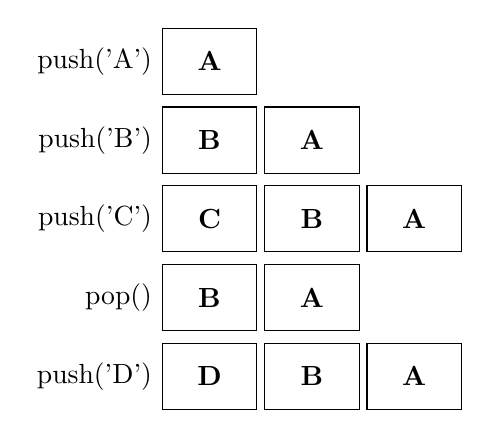
\begin{tikzpicture}[box/.style={draw,rectangle,inner sep=.3cm,node distance=1cm,minimum width=1.2cm,font={\bfseries}}]
		\node[box,label=left:{\code{push('A')}}] (A1) {A};
		\node[box,below of=A1,label=left:{\code{push('B')}}] (B1) {B};
		\node[box,right of=B1,xshift=.3cm] (A2) {A};
		\node[box,below of=B1,label=left:{\code{push('C')}}] (C1) {C};
		\node[box,right of=C1,xshift=.3cm] (B2) {B};
		\node[box,right of=B2,xshift=.3cm] (A3) {A};
		\node[box,below of=C1,label=left:{\code{pop()}}] (B3) {B};
		\node[box,right of=B3,xshift=.3cm] (A4) {A};
		\node[box,below of=B3,label=left:{\code{push('D')}}] (D1) {D};
		\node[box,right of=D1,xshift=.3cm] (B4) {B};
		\node[box,right of=B4,xshift=.3cm] (A5) {A};
	\end{tikzpicture}
	\end{center}
\end{aufgabe}

\begin{aufgabe}[icon=\Large\iconPartner]
	Die hier vorgestellte Datenstruktur wird in der Informatik als
	\emph{Stapel} (englisch \emph{Stack}) bezeichnet. Ein Stapel arbeitet nach
	dem Verarbeitungsprinzip \enquote{\emph{Last in - First out}} (\emph{LIFO}).

	\begin{teilaufgaben}
		\teilaufgabe Erklärt die Herkunft der Bezeichnung \enquote{Last In -
		First Out} anhand der Darstellungen aus Aufgabe 1 bis 3.
		\teilaufgabe Beschreibt das \emph{LIFO}-Prinzip mit eigenen Worten.
	\end{teilaufgaben}

	\begin{center}
	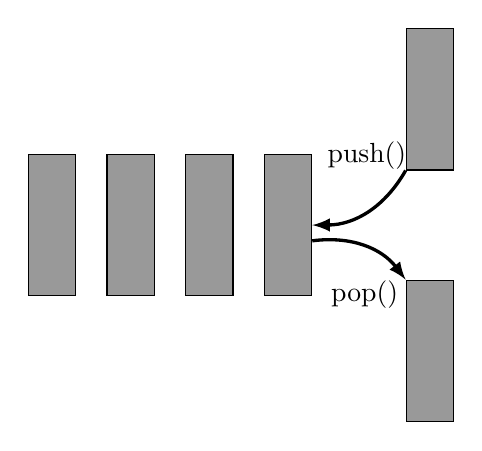
\begin{tikzpicture}[box/.style={draw,rectangle,fill=black!40,minimum width=.6cm,minimum height=1.8cm}]
		\node[box] (b1) {};
		\node[box,right of=b1] (b2) {};
		\node[box,right of=b2] (b3) {};
		\node[box,right of=b3] (b4) {};
		\node[box,right of=b4,xshift=.8cm,yshift=1.6cm] (b5) {};
		\node[box,right of=b4,xshift=.8cm,yshift=-1.6cm] (b6) {};
		\path[->,>=latex,auto,very thick] (b5.south west) edge[bend left] node [above,yshift=.4cm] {\code{push()}} (b4.east)+(0,.2);
		\path[->,>=latex,auto,very thick] (b4.east)+(0,-.2) edge[bend left] node [below,yshift=-.3cm] {\code{pop()}} (b6.north west);
	\end{tikzpicture}
	\end{center}
\end{aufgabe}

\end{document}
